\section{Implementation} \label{section-implementation}

Several software components were developed to implement a server push service for the Tsuru platform.

The development strategy adopted was to first develop the more independent components, and add extra layers of complexity or integration later. So the development followed these steps, which will be examined in detail next:
\begin{itemize}
    \item develop the Push Service, a micro-services based system to provide a server push service on top of the Nginx Push Stream module.
    \item develop the PushaaS system, with the capability of provisioning instances of Push Service in response to a service call.
    \item deploy the whole ecosystem to a cloud infrastructure and integrate the PushaaS with a Tsuru cluster, in order to perform tests and evaluate the implementation.
\end{itemize}


\subsection{Push Service}

The Push Service was developed as a micro-services system to augment the Nginx Push Stream module capabilities, by enabling a more scalable architecture, a more flexible deployment and a layer of extra functionality for users.

It helps to understand the role played by the Push Service once the limitations of the simple use of the Nginx Push Steam module are understood. The module works by being compiled together with the Nginx code, and this compilation results in a binary with the Nginx server with the Push Stream enabled. An instance of Nginx with Push Stream module could be run and configured to provide the server push functionality, by enabling on the Nginx both a publishing endpoint and a subscribing endpoint. This could be enough for very simple scenarios, but presents shortcomings for more complex needs. The main shortcoming is that horizontal scalability is not supported. While multiple instances of Nginx with the module could be deployed, there is no built-in coordination mechanism that would make all the instances work in collaboration. Even if a load balancer is used to distribute clients connecting to the subscribing endpoint, there is still no mechanism for coordinating and synchronizing the publishing of content across all instances. Besides this shortcoming, another aspect is that, while access to the publishing interface can be limited via configuration to only be allowed from specific networks, the module does not offer authentication on the publishing endpoint.

At a high-level, the Push Service can be understood as a publish-subscribe system between instances of a message-publishing interface (accessed by applications operated by a user responsible for publishing content, like some content management system) and a message-consuming interface (accessed by content consumers, typically end-users of some web application).

The Push Service is composed of four different software components, that can be seen in Figure~\ref{fig:push-service}. Briefly, the four components can be summarized as:
\begin{itemize}
    \item push-api~\footnote{https://github.com/pushaas/push-api}: acts as the publishing interface of the system. Applications that want to interact with the Push Service call the push-api HTTP API. The push-api then publishes the received messages to the push-redis.
    \item push-redis~\footnote{https://github.com/pushaas/push-redis}: acts as a publish-subscribe bus and as a data store.
    \item push-agent~\footnote{https://github.com/pushaas/push-agent}: subscribes to messages on the push-redis, an upon a message, publishes it to the associated push-stream instance.
    \item push-stream~\footnote{https://github.com/pushaas/push-stream}: receives subscriptions from end-users, and accepts publication from its associated push-agent instance.
\end{itemize}

\begin{figure}
	\caption{Push Service basic architecture}
	\label{fig:push-service}
	\centering%
	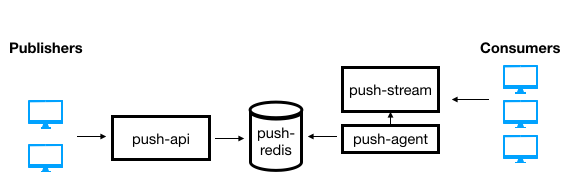
\includegraphics[width=\linewidth]{images/push-service.png}
	\fonte{The author}
\end{figure}

Figure~\ref{fig:push-service} showed the basic architecture of the Push Service, with a single instance of each component. The components could be replicated in order to achieve higher availability or to support higher loads, and load balancers could be added to distribute the load between the system interfaces, like shown in Figure~\ref{fig:push-service-scaled}.

\begin{figure}
	\caption{Push Service scaled}
	\label{fig:push-service-scaled}
	\centering%
	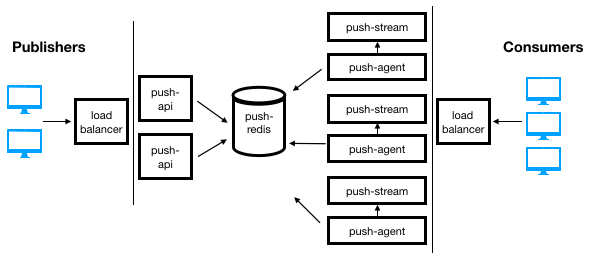
\includegraphics[width=\linewidth]{images/push-service-scaled.png}
	\fonte{The author}
\end{figure}

Now the specific components will be examined in greater detail.


\subsubsection{push-stream}

The Nginx Push Stream module is an open-source third party module for the Nginx web server. It is a mature tool, used by large real-life applications to enable server push functionality. But the plain usage of the module does not answer needs of horizontal scalability and coordination between instances that large applications require.

The Nginx Push Stream module works with the abstraction of channels, where messages can be published to or consumed from. A channel is a logical isolation of messages, providing some kind of scoping for messages. For instance, on a news website, each web page that requires real-time updates could be represented by a different channel.

An instance of Nginx with the Push Stream module installed will accept subscriber connections on channels, and, upon publication of messages on those channels, will distribute the message to all subscribers. The computational power of this instance will determine the number of existing channels, connected subscribers and published messages that the system can handle at once, and the module does not provide any means of horizontal scalability.

Is important to notice that the channels on the Push Stream module are ephemeral. They are allocated when a message is published on them, and consumers can subscribe to them while they exist. But after around 15 minutes of inactivity, they are deallocated and cease to exist, and attempts to subscribe to them will fail. If a persistent channel is to be provided, it must be kept alive with periodic messages just to keep the connections open. The Push Service as a whole provides this functionality of persistent channels, that will be explained on the push-api item.

The number of existing channels tends to pose a lesser problem in real-life applications, because it is usually associated with a dependent business resource, like a channel per different web page, so it doesn't tend to outgrow. But the number of connected subscribers in large applications can easily reach from thousands to millions of users. If multiple instances of the Nginx with Push Stream module were to be deployed to handle this load, a load balancer could be placed in front of the instances and distribute the subscribers between them. But because the load balancing is channel-agnostic, every instance should hold information of every channel, and message publishing should be replicated across all instances, so each instance could notify its subscribers. The Nginx Push Stream module does not provide means for this publishing replication across instances, nor the Push Service system provides the load-balancing capacity in the proposed implementation, but its architecture makes it viable to implement.

The push-stream component of the Push Service is a custom build of the Nginx web server, compiled with the Push Stream module, and a custom configuration file to expose the publishing and subscribing interfaces on Nginx. A very simple configuration exposing the publish-subscribe interface was added, and used to generate a Docker image for this component. The push-stream component does not overcome the limitations presented by the Nginx Push Stream module, only provides a basic Nginx build with the module, which, in coordination with the other components of the Push Service, will be used to overcome such limitations.

The Nginx with Push Stream module exposes routes both for publishing and subscribing to channels. The configuration file provided in the build of the push-stream component should be such that the subscribing interface is exposed and allowed for the targeted users (usually users of a public website), while the the publishing interface should only be exposed to the push-agent component (explained in the next item) corresponding to the push-stream instance.


\subsubsection{push-agent}

The push-agent is a component designed to work as a sidecar application to the push-stream, in order to better integrate it and coordinate with other parts of the system. It consists of a program that, while executed in a different machine or container than the push-stream itself, should guard a one-to-one relationship with the instances of push-stream of the system. For each instance of push-stream deployed, there should be deployed a corresponding push-agent instance, connected to that push-stream instance.

The push-agent is a small program developed in Go, aiming for a small binary with good runtime performance and low resource footprint. It fulfills a twofold role in the system:
\begin{itemize}
    \item it subscribes to the push-redis waiting for messages. When a message arrives, push-agent publishes the message to the publishing interface of its corresponding push-stream instance. The messages were modeled as containing the message data and a list of channels to which publish this data. In most scenarios a message would be published only to a single channel, but this opens some possibilities for optimization of persistent channels, that will be explored later.
    \item it polls the push-stream for status and statistics, and save this data on the push-redis, giving visibility of this data separated by push-agent instances.
\end{itemize}

The existence of the push-agent listening to a bus that notifies message publishing events is a solution for coordinating message publishing across multiple push-stream instances, in the case of multiple instances being used to provide horizontal scalability.


\subsubsection{push-redis}

The Push Service system needs both a data storage system to store information about persistent channels, and a publish-subscribe mechanism to communicate message flow from push-api instances to push-stream instances (through the corresponding push-agent instances). The Redis data store was chosen because it can fulfill both these roles, with high performance and low resource footprint.

The push-redis component is essentially a Docker image of a simple Redis with extra configuration. By default, Redis provides memory-only storage, but to better tolerate failures, the configuration provided activates on-disk storage. This way, in the case of a failure, the persistent channels data are safely stored on disk and can be recovered upon a restart.


\subsubsection{push-api}

It was said on the push-stream item that the Nginx with the Push Stream module provides a publishing interface. But, because of the need of scaling horizontally the push-stream instances, the access to that interface was limited to a corresponding push-agent associated with the push-stream instance. In that way, feeding new messages to the push-agent instances is done by listening to the push-redis. The missing part so far is the publishing interface that can be called by the application that wants to deliver messages to its clients, and this role is played by the push-api.

The push-api is a Go program that both exposes an HTTP API and runs a background worker. The HTTP API exposes to client applications the ability to create and maintain persistent channels, and to publish messages on the channels. The background worker is responsible for keeping the persistent channels alive.

The HTTP API exposed by the push-api interacts with the push-redis. In the case of a channel creation or deletion, a corresponding record is added or removed to the Redis storage. Since Redis provides key expiration out of the box, it was trivial to implement a time-to-live functionality that can be configured on channels on its creation.

In the case of message publishing, the push-redis is used not as storage, but as a the bus. Hence, a message published on a push-api instance is delivered to the push-redis, which acts as a bus and notifies all listening push-agent instances, which in turn publish the message to its corresponding push-stream instance.

In most real-life scenarios, the publishing interface of the system should have a lower load when compared to the subscribing interface (i.e., usually on most systems there are more users consuming content than publishing content). Nonetheless, the push-api is a stateless application and might be easily horizontally scaled, simply by adding a load balancer in front of multiple instances, as long as they all publish messages to the same push-redis instance.

The Push Stream module does not provide authentication, and this might allow for unintended users publishing messages. In the setup proposed in the Push Service, this is acceptable because the Nginx configuration should only allow message publishing coming from the corresponding push-agent instance. But since in the Push Service the publishing surface is extended from the push-stream to the push-api, support for authentication was implemented on the push-api so that only authorized applications can publish content. Currently only HTTP basic authentication support was implemented, but several authentication methods could be easily implemented and made available through configuration.

Besides the HTTP API, the push-api is also composed by the aforementioned background worker. The worker is responsible for keeping alive the channels that were created to be persistent, overcoming the limitation of ephemeral channels imposed by the Push Stream module. The worker runs periodically and checks all channels saved on the push-redis. It then publishes a single message to the push-redis pub-sub system, containing the list of all channels to revive, and a well-known message data that represents a keep-alive message. Later, each instance of push-agent listening to the push-redis will receive the message containing all the channels, and will publish the keep-alive message to its corresponding push-stream instance, on all channels.

The push-api also serves the Push Service Admin, a web application containing an admin interface for the Push Service instance that can be accessed by the appropriated route on the push-api. The Admin application can be accessed using the same credentials that are used to interact with the push-api. The Admin application consists of an overview of the Server Push service. There is a main dashboard with information and statistics that each push-agent stores on the push-redis, and there is a list of all the persistent channels stored on the system. Information about each persistent channel can be seen, such as expiration date (if set), number of connected subscribers and others. Also, a view of messages being published on the channel through the push-api can be seen, as well as an interface for sending messages from the Admin, to be used for debugging purposes.


\subsection{PushaaS}

The PushaaS is the system responsible for provisioning instances of a complete Push Service (with all its four components) in response to a service call made by a developer who wants to create a new Push Service instance to be used by his application.

It consists of a Go program called pushaas~\footnote{https://github.com/pushaas/pushaas} that exposes an HTTP API and runs some background jobs. It also requires a Redis instance to be used both as storage for instances information and to be used as a queue for background jobs.

The HTTP API exposes routes that allow clients to request instances of the Push Service to be provisioned and deprovisioned, as well as other operations like binding the service to applications, which will be further explored on the item about Tsuru Service API.

Upon a call to the appropriate route, the pushaas system will create a job to provision new infrastructure. To make the system more flexible and able to work on different environments and setups, pushaas internally works with the abstraction of provisioners, which are software components that implement a common interface with provision and deprovision methods, and are responsible for taking the appropriate actions on a corresponding infrastructure provider in order to provision or deprovision resources for a Push Service instance on that infrastruture provider.

The infrastructure provisioner choice was implemented as a pushaas application-level configuration, so different organizations using the pushaas system could choose to provision Push Service instances on the infrastructure provider of their choice, like on many public cloud offerings (Amazon EC2, Google Cloud Platform, Microsoft Azure, Digital Ocean) as well as on on-premises solutions (Apache CloudStack, OpenStack). For simplicity, it is an application-level configuration, not a per Push Service instance configuration (i.e., all Push Service instances created via the pushaas will be provisioned on the same infrastructure provider, through the application-level configured provisioner). Currently only a single infrastructure provisioner (Amazon ECS) is implemented, and the default configuration uses it, but the addition of new implementations to the codebase should be trivial.

To provide greater flexibility, the pushaas supports the concept plans for the service. Plan is a concept from Tsuru services, that will be further explored in a later section, but it essentially refers to the amount of computational resources allocated for a service. The pushaas was developed with support for plans, but the current implementation only supports a default "small" plan.

Besides the HTTP API, a web application containing an admin interface for the pushaas was developed, and can be accessed by the appropriated route on the pushaas. The admin application can be accessed using the same credentials that were used to register the service on the Tsuru cluster, and it consists of a tool for administrators to have a unified view of all the Push Service instances provisioned using the PushaaS, and their associated resources.


\subsubsection{Amazon ECS Provisioner}

The role of the provisioner is to create (or remove) resources for a complete Push Service instance to be fully operational, so it can later be bound to an application that will use the service it provides.

The Amazon ECS (Elastic Container Service) was chosen to be the infrastructure provider used to implement the default provisioner, to validate and evaluate the pushaas system, because it offers a light-weight container system with low cost that was convenient for the validation purpose.

Amazon ECS works upon a few important concepts that will be used on the provisioning process:
\begin{itemize}
    \item cluster: is a logical grouping of tasks and services. Tasks and services are defined inside of the scope of a cluster.
    \item task definition: is a description of an abstract task, containing information like the required resources (CPU, memory) for the task, environment variables and containers definitions. A single task definition can be composed of multiple different containers, if needed.
    \item service: is an actual execution of a task. A service is defined inside a cluster, and runs a configured number of instances of a task definition, exposing network addresses for the instances.
    \item service discovery service: to allow services to be referenced by names (instead of IPs) internally on the AWS private network (which is a more convenient and flexible way of referencing services), it is necessary a service discovery mechanism that allow services to be registered by name, creating an indirection to their actual addresses.
\end{itemize}

The provisioning of a new Push Service instance with the Amazon ECS provisioner on pushaas follows these main steps:
\begin{itemize}
    \item the instance data is stored on the pushaas Redis instance, containing information like its name, status and owner team.
    \item provision the Push Service push-redis.
        \begin{itemize}
            \item all instances of Push Service can reuse the same task definition, since there is no custom configuration per different instance. So the task definition for the push-redis was previously created once.
            \item a service discovery service is created so the new push-redis service can be referenced internally by other components by its service name.
            \item a service is created using the task definition and the service discovery service. The service is created with the appropriated security groups and on the appropriate subnet.
            \item the system waits for the service to become on the "running" state.
        \end{itemize}
    \item provision the Push Service push-stream and push-agent.
        \begin{itemize}
            \item a specific task definition is created for this instance of Push Service. This task definition defines that is composed of two containers, one from the push-stream image and one from the push-agent image. The push-agent definition receives environment variables that define the appropriate addresses to connect to the corresponding push-stream and to the push-redis of the Push Service instance.
            \item a service discovery service is created so the new push-stream service can be referenced internally by other components by its service name,
            \item a service is created using the task definition and the service discovery service. The service is created with the appropriated security groups and on the appropriate subnet.
            \item the system waits for the service to become on the "running" state.
        \end{itemize}
    \item provision the Push Service push-api.
        \begin{itemize}
            \item a specific task definition is created for this instance of Push Service. This task definition defines that is composed of one container from the push-api image. The container definition receives environment variables that define the appropriate address to connect to the push-redis of the Push Service instance, as well as generated credentials to be used by applications to connect to the push-api instance, and the public address for clients who want to connect to the push-stream. Here there is a point of technical debt that was overlooked for sake of simplicity on the current implementation. End-user applications who want to receive real-time updates must be connected to the push-stream component to receive the updates. These applications can know the address of the push-stream to connect by asking the push-api on the appropriate route. The technical debt is that, since currently no load balancers are being added in front of the push-stream component (because in the existing small plan there is only a single instance of each component), the push-stream service is being exposed publicly and its public IP is being used for clients to connect, which is less flexible than in ideal situation where a load balancer would abstract these details from the client application.
            \item a service discovery service is created so the new push-api service can be referenced internally by other components by its service name.
            \item a service is created using the task definition and the service discovery service. The service is created with the appropriated security groups and on the appropriate subnet.
            \item the system waits for the service to become on the "running" state.
        \end{itemize}
    \item the instance data is updated with the running status, so users can query and know that the provisioning is done.
\end{itemize}

Since the pushaas supports plans, but only a "small" plan is currently implemented, all instances of the Push Service are being provisioned with the same amount of computational resources. The current implementation creates only a single instance of each component and does not add load balancers in front of the push-api or the push-stream. This was done to simplify the process of provisioning in the current state of development of the project, but poses a limitation that should be solved in a future development to allow for greater flexibility and scalability. All containers in the "small" plan are created with 256 CPU units (a computational resource measurement used on AWS ECS), and 512 MiB of memory.


\subsubsection{Tsuru Service API}

The pushaas as explained so far has the ability to provision and deprovision Push Service instances. But this work intends to offer this functionality as a Tsuru Service.

The process of integrating a service to a Tsuru cluster is trivial:
\begin{itemize}
    \item the service must be registered on the Tsuru cluster.
    \item the service must offer some HTTP routes that will be called when the Tsuru user interacts with the service.
\end{itemize}

Registering the service on the Tsuru cluster is done by creating a manifest file that configures service informations (like endpoints and credentials) and running the appropriate commands on the Tsuru CLI~\footnote{https://docs.tsuru.io/1.7/services/build.html\#creating-a-service-manifest}.

Since this service was planned from the beginning to be integrated to Tsuru, the routes for service instances provisioning were created following the Tsuru Service API Specification~\footnote{https://docs.tsuru.io/1.7/services/api.html#api-specification}. Besides the routes for provisioning, to fulfill the specification, some routes are needed for binding service instances to applications. The process of binding consists basically of:
\begin{itemize}
    \item tracking internally that the service instance is related to a given application.
    \item returning a set of environment variables that will be set on the application, with information the application needs to reach the service (like endpoints and credentials).
    \item taking any kind of extra actions, like allowing network access to resources. In the current setup and with the AWS ECS provisioner, no extra actions were required.
\end{itemize}

All the provisioning and binding functionality was developed and exposed accordingly to the Tsuru Service API Specification, and with the service registration, the service was exposed as a Tsuru service.


\subsection{Infrastructure on AWS}

To validate the implementation of the whole PushaaS system (the deployment of the pushaas app, the integration with Tsuru applications and the provisioning of Push Service instances), it is necessary to deploy the system as a whole to some infrastructure.

The main components that need to be deployed are:
\begin{itemize}
    \item the Tsuru cluster, with control nodes - where Tsuru runs its own internal components, and with poll nodes - where the client applications get deployed.
    \item the pushaas app, and its Redis instance.
    \item the Push Service instances that get provisioned upon calls to the pushaas API.
\end{itemize}

The chosen infrastructure provider for this validation was AWS, and Terraform was used to automate processes and achieve better reproducibility~\footnote{https://github.com/pushaas/pushaas-aws-ecs-config}. Figure~\ref{fig:pushaas-infrastructure} shows the overview of the architecture used in the evaluation of the system, presenting the Tsuru cluster, the PushaaS system deployed on Amazon ECS, and instances of the Push Service provisioned on Amazon ECS and bound to applications running on the Tsuru cluster, being accessed by end-users. Note that in the figure, instances of push-agent are not represented explicitly, but represented unified with its associated push-stream instance, for simplicity.

\begin{figure}
	\caption{PushaaS Infrastructure}
	\label{fig:pushaas-infrastructure}
	\centering%
	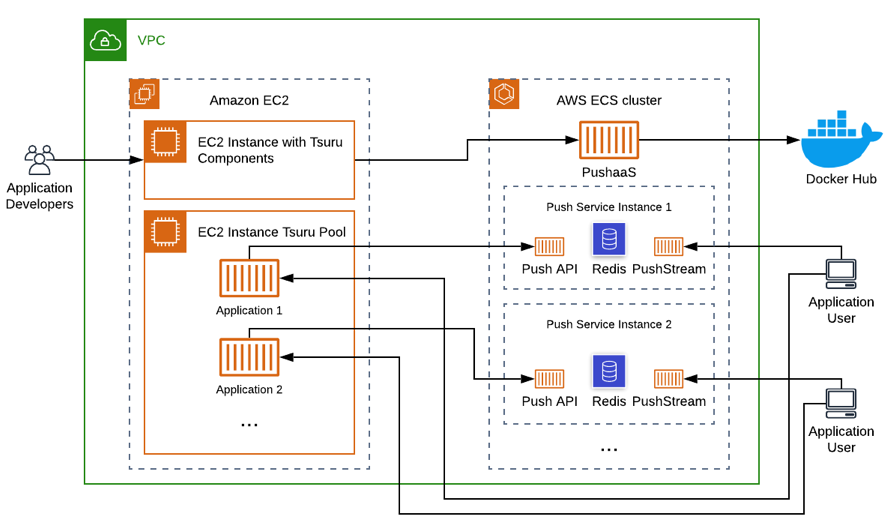
\includegraphics[width=\linewidth]{images/pushaas-infrastructure.png}
	\fonte{The author}
\end{figure}

The main components of infrastructure needed to deploy and validate the PushaaS system will be examined now. The following list contains the main steps taken to deploy the system:
\begin{itemize}
    \item a VPC (virtual private cloud) was created, so the PushaaS system could be all deployed to a single isolated virtual private cloud inside AWS infrastructure.
    \item Tsuru was installed on Amazon EC2. The Tsuru installer was used, and it created a virtual machine for the Tsuru components, and a separate machine to be the Tsuru pool, where applications get deployed. Since it was a simple validation of a integrated service, a pool with a single machine was enough to hold the client applications.
    \item Tsuru roles and teams were configured, so later they could be used to grant permissions to developers during the validation process.
    \item a private DNS namespace was created, to allow for registering DNS records of services, so services could be addressed by their names instead of IPs.
    \item an Amazon ECS cluster was created, to hold task definitions and services that would later be created.
    \item an ECS service was created running an instance of Redis, to be used by the pushaas.
    \item an ECS service was created running the pushaas.
    \item the pushaas ECS service address was used to generate a manifest file and register the service on the Tsuru cluster.
    \item an ECS task definition for the push-redis was created, as noted previously that since all instances of Push Service would run an exact copy of the same push-redis image, the task definition could be shared among all instances.
    \item the NodeJS platform was added to the Tsuru cluster. This makes Tsuru capable of running NodeJS applications. The test application develop for the validation process is a NodeJS application, so it could now be deployed and run on Tsuru.
\end{itemize}
